%TCIDATA{LaTeXparent=0,0,cap_RevisaoBibliografica.tex}

\section{Métodos Convencionais de Recuperação Secundária}

\subsection{Conceito e Contextualização da Recuperação Secundária}

De acordo com Rosa, nas acumulações de petróleo há, na época de sua descoberta, uma dada quantidade de energia, chamada de \textit{energia primária}, cuja grandeza é determinada pelo volume e pela natureza dos fluidos existentes no meio, além dos níveis de pressão e temperatura do reservatório. Quando se dá o processo de produção, parte dessa energia é dissipada por causa da descompressão dos fluidos do reservatório e das resistências que os mesmos encontram ao fluir em direção aos poços produtores --- resistências associadas às forças viscosas e capilares presentes no meio poroso. A consequência dessa dissipação de energia primária resulta no decréscimo de pressão do reservatório em sua vida produtiva e, consequentemente, na redução da produtividade dos poços. A quantidade de óleo retirada utilizando-se unicamente a energia do reservatório é denominada \textit{recuperação primária}.

De forma a se minorar os efeitos danosos da dissipação da energia primária, existem duas linhas de ação a serem consideradas:

\begin{itemize}
\item Reduzir as resistências viscosas e/ou capilares por meio de métodos especiais, como por exemplo aquecendo a jazida;
\item Adicionar suplemento de energia secundária, artificialmente comunicada, através de injeção de fluidos em poços selecionados.
\end{itemize}

Quando se suplementa o reservatório com energia transferida artificialmente, ou se empregam meios de incrementar a eficiência da energia primária, a quantidade adicional de óleo produzida é chamada de \textit{recuperação secundária}. Por extensão, todas as operações que conduzem à obtenção desse adicional de óleo também são denominadas recuperação secundária. Essas operações, atualmente, são implantadas em sua grande maioria o tão cedo quanto possível na vida do reservatório.

É importante ressaltar que há uma diferença entre recuperação secundária e métodos de elevação artificial e de estimulação de poços; estes não afetam diretamente as energias expulsivas do reservatório, embora sua aplicação concorra para economizá-las. As técnicas de elevação artificial e de estimulação de poços estão mais ligadas ao comportamento dos poços produtores do que ao comportamento do reservatório como um todo. Contudo, a linha divisória entre tais métodos e os métodos de recuperação secundária não é muito nítida --- certos métodos de estimulação, como a injeção cíclica de vapor, são usualmente incluídos entre os métodos de recuperação secundária \cite{engres}.

Ainda segundo Rosa, há dois objetivos práticos básicos dos métodos de recuperação secundária:

\begin{itemize}
\item \textbf{Aumento da eficiência de recuperação} --- A eficiência de recuperação primária é normalmente baixa; em alguns casos, dependendo das características do reservatório e dos fluidos, ela pode ser até nula. Em alguns casos, a eficiência de recuperação secundária pode passar de 60\% em casos bem-sucedidos; contudo, o valor mais frequente dessa eficiência, nos métodos convencionais, se situa entre 30 e 50\%.
\item \textbf{Aceleração da produção} --- O emprego dos métodos de recuperação secundária busca acelerar a produção ou ao menos reduzir a taxa de seu declínio natural. A aceleração da produção resulta em antecipação do fluxo de caixa; portanto, há o aumento de seu valor presente e uma consequente melhoria da economicidade da exploração do campo ou reservatório.
\end{itemize}

Além dos objetivos básicos de emprego da recuperação secundária, Rosa citam vários incentivos ao uso desses métodos, tais como: preço do petróleo; custos de exploração, desenvolvimento e produção; e avanços tecnológicos na área. Porém, destaca-se que apenas o uso dessas técnicas não é o suficiente para mitigar todos os males da produção de petróleo e do esgotamento das reservas; outras medidas podem e devem ser tomadas, simultaneamente, para aumentar a eficiência e a rentabilidade da produção, tais como:

\begin{itemize}
\item \textbf{Exploração de reservas não convencionais} --- Xistos e folhelhos betuminosos, por exemplo, acumulam grandes quantidades de óleo. Várias dessas reservas já foram encontradas em regiões como Athabasca, no Canadá, cinturão do Orinoco, na Venezuela, e o Colorado, nos Estados Unidos. O custo de produção nessas reservas é considerável, mas já se projetam meios tecnológicos para reduzir o mesmo. Entre outras reservas não convencionais de hidrocarbonetos, há a presença de gás natural em solução existente na água de aquíferos; embora a razão de solubilidade do gás natural na água normalmente seja pequena, o imenso volume dos aquíferos perimitiria uma produção de grandes volumes desse gás. Uma outra reserva não convecional poderá ser o gás natural proveniente de hidratos localizados no fundo de oceanos e em regiões congeladas da Terra.
\item \textbf{Estimulação de Poços} De acordo com Thomas, a estimulação de poços é um conjunto de atividades realizadas com o objetivo de aumentar o índice de produtividade ou injetividade do poço \cite[p.~166]{engpetro}. Os principais métodos de estimulação são: fraturamento hidráulico, em que se cria, através de uma ruptura na rocha-reservatório causada por um elevado gradiente de pressão, um caminho preferencial de alta condutividade, facilitando um fluxo de fluidos do reservatório ao poço (ou vice-versa); e acidificação, onde se injeta um ácido com pressão inferior à pressão de fraturamento da formação, visando remover danos da mesma. Tais métodos contribuem para a aceleração da produção e até, em alguns casos, o aumento da eficiência de recuperação. A aplicação de métodos de estimulação pode, inclusive, ser feita em campos submetidos a operações de recuperação secundária.
\item \textbf{Uso de poços especiais} --- Nas últimas décadas houve um incremento considerável no uso dos chamados \textit{poços especiais}, que possuem como característica marcante a não-verticalidade, Segundo Thomas, esses poços são perfurados com várias finalidades, como: controlar um poço em \textit{blowout} por meio de poços de alívio; atingir formações produtoras abaixo de locais inacessíveis, como rios, lagos, cidades, entre outros; desviar a trajetória do poço de acidentes geológicos, como domos salinos e falhas; perfurar vários poços de um mesmo ponto, como é o caso da produção em plataformas marítimas; e desviar poços que tiveram seu trecho final perdido por problemas operacionais \cite[p.~106]{engpetro}. O uso desses poços inclinados, horizontais, multilaterais, etc., pode aumentar a velocidade de drenagem do reservatório, ou seja, antecipar a produção, bem como aumentar a eficiência de recuperação através do aumento da eficiência de varrido, por exemplo.
\item \textbf{Extração de líquidos de gás natural} --- A produção de hidrocarbonetos líquidos pode ser aumentada pela instalação de plantas de gasolina natural e de unidades portáteis de extração de líquidos de gás natural.
\item \textbf{Reestudo de áreas julgadas improdutivas ou antieconômicas} --- Mesmo que as reservas mundiais de petróleo sejam limitadas, elas estão longe de terem sido totalmente exploradas; de fato, apenas uma pequena porcentagem da superfície do planeta foi inteiramente explorada. Seja na terra ou no fundo do mar, há ainda perspectivas notáveis fora das áreas hoje em produção; além disso, as estimativas do volume de óleo que ainda poderá ser descoberto são ainda vagas. É com essa perspectiva que a indústria pode medir as oportunidades que tem à frente no caso de esgotamento das áreas hoje em produção. Portanto, de um modo geral, deve-se pensar sempre na adoção das seguintes medidas, sem danos ao andamento das operações de recuperação secundária: estudar novas áreas; estudar formações mais profundas (o pré-sal é um exemplo); reestudar áreas consideradas esgotadas ou de produção antieconômica; e investir mais dinheiro, tempo e pessoal em treinamento e pesquisa, visando melhorar os métodos de exploração e produção existentes.
\end{itemize}

\subsection{Classificação dos Métodos de Recuperação Secundária}
Segundo Rosa, os métodos de recuperação de óleo visando suplementar a energia do reservatório, logo após a fase de recuperação primária, eram denominados, originalmente, métodos de recuperação secundária, enquanto que logo após essa fase de recuperação secundária eram empregados outros métodos, chamados de \textit{recuperação terciária}. Os métodos eram então classificados de acordo com a sua cronologia de aplicação em determinado campo ou reservatório. Posteriormente, todos os métodos de recuperação aplicados com o objetivo de aumentar a eficiência de recuperação e/ou acelerar a produção em relação à produção primária passaram a ser denominados de recuperação secundária\footnote{Ver \cite[p. 564]{engres}.}.

Nas últimas décadas, a classificação dos métodos de recuperação secundária se deu em \textit{métodos convencionais} (os antigos métodos de recuperação secundária) e \textit{métodos especiais} (os antigos métodos de recuperação terciária), os últimos também conhecidos, na literatura inglesa, como métodos de \textit{EOR} (\textit{Enhanced Oil Recovery}) --- esse termo, nos últimos anos, tem sido substituído pelo termo \textit{IOR} (\textit{Improved Oil Recovery}), cuja diferença, em relação ao \textit{EOR}, reside no fato de que os métodos de \textit{IOR} englobam, além dos métodos de \textit{EOR}, quaisquer métodos ou técnicas não-convencionais ou modernas que possuam o objetivo de aumentar a produção e/ou acelerar a produção em relação à produção primária e/ou secundária\footnote{\textit{Ibid.}, p. 564.}. 

Em termos da classificação mais atual, são métodos convencionais de recuperação secundária os métodos de injeção de água e injeção imiscível de gás. Já os métodos especiais incluem, entre outros, a injeção miscível de gás, a injeção de vapor, a injeção de polímeros e a combustão \textit{in situ}\footnote{\textit{Ibid.}, p. 564. Uma abordagem sobre os métodos especiais pode ser encontrada em \cite[pp. 677-726]{engres}}.

\subsection{Métodos Convencionais}
Os dois tipos de métodos considerados convencionais, já citados, são os métodos de injeção imiscível de fluidos no reservatório, seja água ou gás. Segundo Eremin, o método de injeção de água é um dos mais utilizados devido à sua utilização também como método mantenedor da pressão no reservatório, além do fato da água ser um fluido acessível, consideravelmente barato e possuir propriedade de deslocamento específica \cite{eremin}. Já a injeção de imiscível de gás consiste em injeção de fluido gasoso, mas de forma que ele não se misture ao óleo, criando uma mistura bifásica \cite[p. 564]{engres}.

Segundo Rosa, ao se escolher um projeto de injeção, deve-se levar em conta a escolha do esquema de injeção, isto é, da distribuição dos poços de injeção e de produção mais adequada ao reservatório de petróleo em estudo. Como o objetivo primordial da injeção é o aumento da recuperação de petróleo, deve-se tentar produzir esse volume adicional desejado utilizando-se esquemas em que os volumes de fluidos injetados sejam os menores possíveis e a produção do fluido injetado seja a menor possível. Por fim, devem ser observadas as características particulares do reservatório em estudo, como a existência de falhas, variações de permeabilidade, etc., além do aspecto econômico da produção \cite[p. 564]{engres}; o aspecto econômico envolve estudo de custos relacionados à adoção do método de recuperação, como os custos de estudo, de perfuração de novos poços, da conversão de poços produtores em injetores, entre outros \cite{latil}.

De acordo com Latil, entre os métodos convencionais de injeção de fluidos, o de injeção de gás é mais indicado em casos de reservatórios com baixa razão gás-óleo --- neste caso, seria necessária um grande volume de gás injetado para se criar a fase gasosa --- ou de óleo saturado, desde que a permeabilidade à água seja suficientemente alta; já em casos de reservatórios com alta razão gas-óleo, a injeção imiscível de gás se torna um método que resulta em melhores índices de recuperação de óleo. Por fim, em casos de reservatórios heterogêneos com presença de água, a injeção de água é a mais recomendada \cite{latil}. 

\subsection{Esquemas de Injeção}
Segundo Rosa, há vários tipos de esquemas de injeção, separados em dois grupos principais: os esquemas baseados na estrutura do reservatório (injeção periférica, no topo ou na base) ou baseados no modo como os poços são distribuídos (esquemas em malha) \cite[p. 564]{engres}.

\subsubsection{Esquemas baseados na Estrutura do Reservatório}
Nos esquemas baseados na estrutura do reservatório, os poços de mesmo tipo (de injeção ou de produção) se concentram em determinadas áreas do reservatório. Em reservatórios de estrutura anticlinal, por exemplo, é mais utilizado o esquema de \textit{injeção periférica}, mostrada na Figura \ref{fig:rev_injper}. Neste caso, os poços produtores se concentram no centro do reservatório, equanto que os injetores são situados na periferia do mesmo, justificando o nome do esquema\footnote{Ver \cite[p. 565]{engres}}. A \textit{injeção no topo} consiste em situar os poços injetores no topo do reservatório, enquanto os produtores são localizados na base (ver Figura \ref{fig:rev_injtop}); o fluido injetado, neste caso, é o gás. Por fim, a \textit{injeção na base} considera os poços injetores na base do reservatório e os produtores no topo (ver Figura \ref{fig:rev_injbas}); o fluido injetado, neste caso, é a água. Vale notar que os esquemas de injeção no topo e na base podem ser combinados, e que, em determinado momento, os poços produtores podem ser convertidos em poços injetores. Rosa ainda destaca que, na verdade, essas diferentes maneiras de se fazer injeção não se classificam exatamente como
\textit{esquemas} de injeção, uma vez que a disposição dos poços não está previamente estabelecida, ou seja, não existem arranjos prefixados para a localização dos poços \cite[p. 566]{engres}.

\begin{figure}[!ht]
\centering
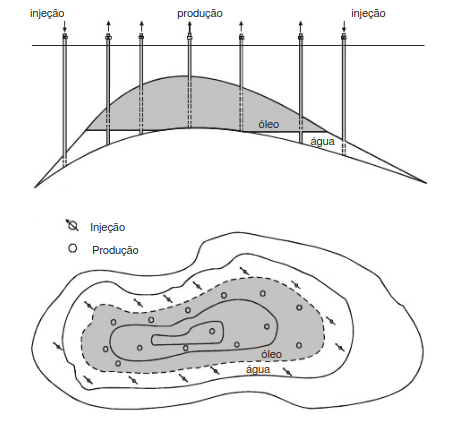
\includegraphics[width=.6\textwidth]{figs/revisao/revisao_injper.png}
\caption{Injeção periférica \cite[p. 565]{engres}.}
\label{fig:rev_injper}
\end{figure}

\begin{figure}[!ht]
\centering
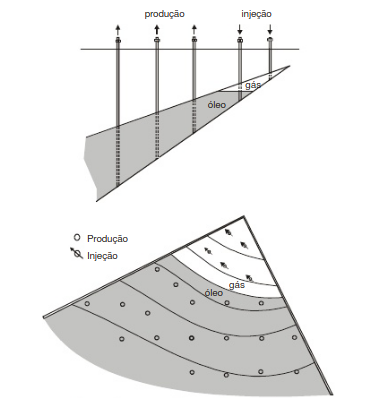
\includegraphics[width=.6\textwidth]{figs/revisao/revisao_injtop.png}
\caption{Injeção no topo \cite[p. 566]{engres}.}
\label{fig:rev_injtop}
\end{figure}

\begin{figure}[!ht]
\centering
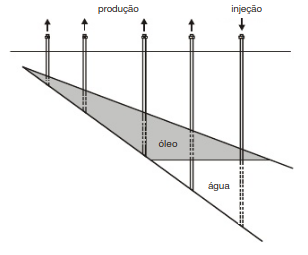
\includegraphics[width=.6\textwidth]{figs/revisao/revisao_injbas.png}
\caption{Injeção na base \cite[p. 566]{engres}.}
\label{fig:rev_injbas}
\end{figure}





\subsubsection{Esquemas de Injeção em Malha}
Neste grupo, se situam esquema de injeção aplicados em reservatórios com grandes áreas e pequenas inclinações e espessuras; os poços tanto de um tipo quanto do outro estão uniformemente distribuídos em toda a área do reservatório. Neste caso, o fluido deslocante é injetado na própria zona de óleo, alterando-se drasticamente a distribuição de saturações e a movimentação natural dos fluidos no reservatório \cite[p. 567]{engres}.

Dos tipos de injeção em malha, destacam-se as injeções em \textit{linha direta} e em \textit{linhas esconsas}, em que, os poços de produção e injeção são alternados em linhas, formando malhas normalmente retangulares; no caso das linhas esconsas, há uma defasagem entre as linhas de produtores e injetores. As Figuras \ref{fig:rev_injld} e \ref{fig:rev_injle} mostram, respectivamente, exemplos de esquemas de linha direta e linhas esconsas.

\begin{figure}[!ht]
\centering
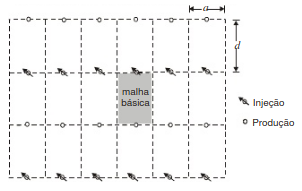
\includegraphics[width=.6\textwidth]{figs/revisao/revisao_injld.png}
\caption{Injeção em linha direta \cite[p. 567]{engres}.}
\label{fig:rev_injld}
\end{figure}

\begin{figure}[!ht]
\centering
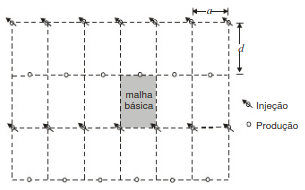
\includegraphics[width=.6\textwidth]{figs/revisao/revisao_injle.png}
\caption{Injeção em linhas esconsas \cite[p. 567]{engres}.}
\label{fig:rev_injle}
\end{figure}

Em alguns casos, os esquemas de malha em linhas diretas ou esconsas podem ser adaptados utilizando-se polígonos regulares como constituintes da malha; três exemplos deste tipo de caso são:
\begin{itemize}
\item \textbf{Malha \textit{five-spot}:} Neste caso, a malha é formada por linhas esconsas, formando um quadrado perfeito; um poço produtor é cercado por quatro injetores (ver Figura \ref{fig:rev_inj5s}).
\item \textbf{Malha \textit{seven-spot}:} A malha considerada consiste em hexágonos regulares, em que um poço produtor é cercado por seis injetores (ver Figura \ref{fig:rev_inj7s}); pode ser considerada um esquema de linhas esconsas, mas com alterância de dois injetores para cada produtor em cada linha.
\item \textbf{Malha \textit{nine-spot}:} Assim como a malha \textit{five-spot}, é constituída por quadrados; porém, o esquema de injeção base pode ser visto como linhas diretas, em que há linhas só de injetores e linhas alternadas entre produtores e injetores; neste tipo de malha, cada poço produtor é cercado por oito poços injetores (ver Figura \ref{fig:rev_inj9s}).
\end{itemize}

\begin{figure}[!ht]
\centering
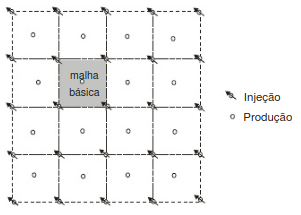
\includegraphics[width=.6\textwidth]{figs/revisao/revisao_inj5s.png}
\caption{Malha \textit{five-spot} \cite[p. 568]{engres}.}
\label{fig:rev_inj5s}
\end{figure}

\begin{figure}[!ht]
\centering
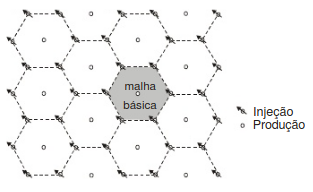
\includegraphics[width=.6\textwidth]{figs/revisao/revisao_inj7s.png}
\caption{Malha \textit{seven-spot} \cite[p. 568]{engres}.}
\label{fig:rev_inj7s}
\end{figure}

\begin{figure}[!ht]
\centering
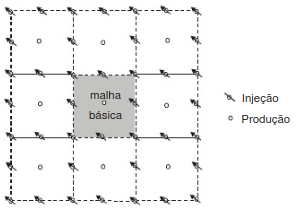
\includegraphics[width=.6\textwidth]{figs/revisao/revisao_inj9s.png}
\caption{Malha \textit{nine-spot} \cite[p. 568]{engres}.}
\label{fig:rev_inj9s}
\end{figure}

Os esquemas de injeção em malhas vistos nas Figuras \ref{fig:rev_inj5s}, \ref{fig:rev_inj7s} e \ref{fig:rev_inj9s} consideram um poço produtor cercado de vários injetores; são consideradas, portanto, malhas de tipo \textit{normal}. Contudo, as mesmas malhas podem também ser projetadas tomando-se em conta um poço injetor cercado por vários produtores; são as chamadas \textit{malhas invertidas} ou \textit{inversas} \cite[p. 569]{engres}. As Figuras \ref{fig:rev_inj7i} e \ref{fig:rev_inj9i} mostram exemplos de malhas invertidas.

\begin{figure}[!ht]
\centering
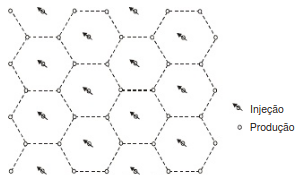
\includegraphics[width=.6\textwidth]{figs/revisao/revisao_inj7i.png}
\caption{Malha inversa \textit{seven-spot} \cite[p. 569]{engres}.}
\label{fig:rev_inj7i}
\end{figure}

\begin{figure}[!ht]
\centering
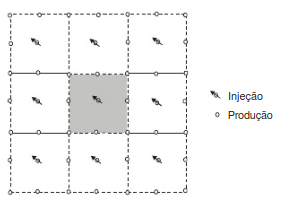
\includegraphics[width=.6\textwidth]{figs/revisao/revisao_inj9i.png}
\caption{Malha inversa \textit{nine-spot} \cite[p. 569]{engres}.}
\label{fig:rev_inj9i}
\end{figure}

\subsection{Aspectos Operacionais da Injeção de Água}
